\documentclass[tikz, border=15pt]{standalone}
\usepackage{amsmath}

\begin{document}
	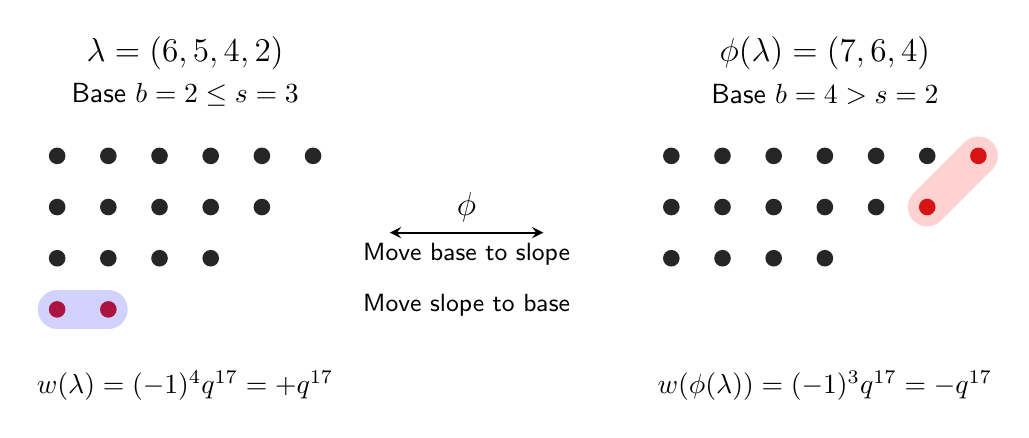
\begin{tikzpicture}[
		scale=0.65,
		dot/.style={circle, fill=black!85, minimum size=6pt, inner sep=0pt},
		active dot/.style={circle, fill=red!80!black, minimum size=6pt, inner sep=0pt},
		base highlight/.style={blue!70, line width=14pt, opacity=0.25, line cap=round},
		slope highlight/.style={red!70, line width=14pt, opacity=0.25, line cap=round}
		]
		
		% ---------------------------------------------------------
		% Left Side: The Original Partition (Even length: 4 parts)
		% ---------------------------------------------------------
		\begin{scope}[xshift=0cm]
			\node[font=\sffamily\large] at (3.5, 6) {$\lambda = (6, 5, 4, 2)$};
			\node[font=\sffamily] at (3.5, 5.2) {Base $b=2 \le s=3$};
			\node[font=\sffamily] at (3.5, -0.5) {$w(\lambda) = (-1)^4 q^{17} = +q^{17}$};
			
			% Draw static dots
			\foreach \y/\n in {4/6, 3/5, 2/4} {
				\foreach \x in {1,...,\n} {
					\node[dot] at (\x, \y) {};
				}
			}
			
			% Draw the active base dots (the ones that will move)
			\node[active dot] at (1, 1) {};
			\node[active dot] at (2, 1) {};
			
			% Highlight the base
			\draw[base highlight] (1,1) -- (2,1);
		\end{scope}
		
		% ---------------------------------------------------------
		% The Mapping \phi (The Involution)
		% ---------------------------------------------------------
		\draw[<->, thick, >=stealth] (7.5, 2.5) -- (10.5, 2.5) 
		node[midway, above, font=\large] {$\phi$}
		node[midway, below, font=\sffamily\small] {Move base to slope};
		
		\draw[<->, thick, >=stealth, color=white] (7.5, 1.5) -- (10.5, 1.5) 
		node[midway, below, font=\sffamily\small, color=black] {Move slope to base};
		
		% ---------------------------------------------------------
		% Right Side: The Mapped Partition (Odd length: 3 parts)
		% ---------------------------------------------------------
		\begin{scope}[xshift=12cm]
			\node[font=\sffamily\large] at (4, 6) {$\phi(\lambda) = (7, 6, 4)$};
			\node[font=\sffamily] at (4, 5.2) {Base $b=4 > s=2$};
			\node[font=\sffamily] at (4, -0.5) {$w(\phi(\lambda)) = (-1)^3 q^{17} = -q^{17}$};
			
			% Draw static dots (same as left side)
			\foreach \y/\n in {4/6, 3/5, 2/4} {
				\foreach \x in {1,...,\n} {
					\node[dot] at (\x, \y) {};
				}
			}
			
			% Draw the active dots in their new slope position
			\node[active dot] at (7, 4) {};
			\node[active dot] at (6, 3) {};
			
			% Highlight the new slope
			\draw[slope highlight] (7,4) -- (6,3);
		\end{scope}
		
	\end{tikzpicture}
\end{document}